% Options for packages loaded elsewhere
\PassOptionsToPackage{unicode}{hyperref}
\PassOptionsToPackage{hyphens}{url}
\documentclass[
]{article}
\usepackage{xcolor}
\usepackage{amsmath,amssymb}
\setcounter{secnumdepth}{-\maxdimen} % remove section numbering
\usepackage{iftex}
\ifPDFTeX
  \usepackage[T1]{fontenc}
  \usepackage[utf8]{inputenc}
  \usepackage{textcomp} % provide euro and other symbols
\else % if luatex or xetex
  \usepackage{unicode-math} % this also loads fontspec
  \defaultfontfeatures{Scale=MatchLowercase}
  \defaultfontfeatures[\rmfamily]{Ligatures=TeX,Scale=1}
\fi
\usepackage{lmodern}
\ifPDFTeX\else
  % xetex/luatex font selection
\fi
% Use upquote if available, for straight quotes in verbatim environments
\IfFileExists{upquote.sty}{\usepackage{upquote}}{}
\IfFileExists{microtype.sty}{% use microtype if available
  \usepackage[]{microtype}
  \UseMicrotypeSet[protrusion]{basicmath} % disable protrusion for tt fonts
}{}
\makeatletter
\@ifundefined{KOMAClassName}{% if non-KOMA class
  \IfFileExists{parskip.sty}{%
    \usepackage{parskip}
  }{% else
    \setlength{\parindent}{0pt}
    \setlength{\parskip}{6pt plus 2pt minus 1pt}}
}{% if KOMA class
  \KOMAoptions{parskip=half}}
\makeatother
\usepackage{graphicx}
\makeatletter
\newsavebox\pandoc@box
\newcommand*\pandocbounded[1]{% scales image to fit in text height/width
  \sbox\pandoc@box{#1}%
  \Gscale@div\@tempa{\textheight}{\dimexpr\ht\pandoc@box+\dp\pandoc@box\relax}%
  \Gscale@div\@tempb{\linewidth}{\wd\pandoc@box}%
  \ifdim\@tempb\p@<\@tempa\p@\let\@tempa\@tempb\fi% select the smaller of both
  \ifdim\@tempa\p@<\p@\scalebox{\@tempa}{\usebox\pandoc@box}%
  \else\usebox{\pandoc@box}%
  \fi%
}
% Set default figure placement to htbp
\def\fps@figure{htbp}
\makeatother
\setlength{\emergencystretch}{3em} % prevent overfull lines
\providecommand{\tightlist}{%
  \setlength{\itemsep}{0pt}\setlength{\parskip}{0pt}}
\usepackage{bookmark}
\IfFileExists{xurl.sty}{\usepackage{xurl}}{} % add URL line breaks if available
\urlstyle{same}
\hypersetup{
  hidelinks,
  pdfcreator={LaTeX via pandoc}}

\author{}
\date{}

\begin{document}

{}

{Statistica}

{Il data science si riduce all'applicazione di metodi statistici, questi
metodi servono a collezionare dati, analizzarli e }{descriverli.}

{Sarà possibile fare inferenze, cioè cercare di trarre delle conclusioni
su una popolazione }{avendo}{~un campione significativo.}

{}

\section{\texorpdfstring{{Data
types}}{Data types}}\label{h.41pjl3u7385g}

{Le variabili possono essere:}

\begin{itemize}
\tightlist
\item
  {Categoriche, rappresentano un gruppo di oggetti, risposte si/no,
  divise a loro volta in:}
\end{itemize}

\begin{itemize}
\tightlist
\item
  {Nominali, i gruppi non possono essere messi in una scala.}
\item
  {Ordinali, i gruppi possono essere messi in una scala.}
\end{itemize}

\begin{itemize}
\tightlist
\item
  {Numeriche, divise in:}
\end{itemize}

\begin{itemize}
\tightlist
\item
  {Discrete}
\item
  {Continue}
\end{itemize}

{}

\section{\texorpdfstring{{Experimental
probability}}{Experimental probability}}\label{h.gft5n92ulwu4}

\begin{itemize}
\tightlist
\item
  {Trial}{: osservazione di un evento e registro il risultato.}
\end{itemize}

{}

\begin{itemize}
\tightlist
\item
  {Esperimento}{: un insieme di trial.}
\end{itemize}

{}

\begin{itemize}
\tightlist
\item
  {Sample space}{: tutti i possibili risultati che posso ottenere.}
\end{itemize}

{}

\begin{itemize}
\tightlist
\item
  {Probabilità}{: rapporto tra l'evento che mi interessa e tutti i
  risultati possibili.}
\end{itemize}

{}

\begin{itemize}
\tightlist
\item
  {Valore atteso}{: valore medio che mi aspetto quando ripeto
  l\textquotesingle esperimento molte volte. Si ottiene sommando i
  prodotti fra probabilità di un certo valore per il valore stesso.}
\end{itemize}

{Per esempio avendo due dadi da 6 facce il valore medio che uscirà sarà
7 perchè è quello con più combinazioni possibili.}

{}

{SALTIAMO DA SLIDE 10 A 15}

{}

\section{\texorpdfstring{{Distribuzione di
probabilità}}{Distribuzione di probabilità}}\label{h.p19ql9hggae4}

{Descrive tutti i valori assunti dalla variabile e ad ciascun valore
associa il conteggio o la probabilità. La distribuzione viene descritta
tramite:}

\begin{itemize}
\tightlist
\item
  {media {[}$\mu$ {]}: }{somma di tutti i valori / numero di valori}{, }
\item
  {varianza: }{misura di quanto la distribuzione è
  ``appiattita''/allargata. }{La somma di tutte le distanze fra
  individuo e media, ciascuna al quadrato / numero di individui}{,}
\item
  {deviazione standard {[}$\alpha${]}}{: radice quadrata della varianza,}
\end{itemize}

{}

\subsubsection{\texorpdfstring{{M}{isure di tendenza
centrale}}{Misure di tendenza centrale}}\label{h.ryfray9l6boy}

{Ecco alcune misure di tendenza centrale:}

\begin{itemize}
\tightlist
\item
  {media}{: come prima,}
\item
  {mediana}{: numero nel mezzo di un dataset ordinato,}
\item
  {moda}{: valore più frequente.}
\end{itemize}

{}

\subsubsection{\texorpdfstring{{Misure di
asimmetria}}{Misure di asimmetria}}\label{h.5di6yf1a5b45}

{Qui la misura principale è la }{skewness}{, cioè se i dati sono
concentrati da un lato preciso. }

{Se }{media \textgreater{} mediana}{~abbiamo una skew }{positiva
}{quindi i }{dati si concentrano verso il lato SX}{~con coda a DX
(valori estremi che spostano la media). Invece è }{negativa }{se }{media
\textless{} mediana}{~e si ha una }{coda verso SX}{.}

{}

\subsubsection{\texorpdfstring{{Misure di
variabilità}}{Misure di variabilità}}\label{h.tgl8isp40aua}

{Ci sono la varianza e la deviazione standard.}

{}

\subsubsection{\texorpdfstring{{Misura di
correlazione}}{Misura di correlazione}}\label{h.63ezrae0336y}

{Misura di quanto due variabili siano correlate tra loro, sia ha:}

\begin{itemize}
\tightlist
\item
  {Covarianza}
\item
  {Correlazione lineare}{: esiste il metodo su pandas, valore compreso
  fra -1 e 1, più è vicino a 1 più c'è correlazione (si seguono), più è
  vicino a -1 c'è correlazione opposta (prendono `strade diverse') e con
  0 non c'è tipo di correlazione.}
\end{itemize}

{In un scatter plot sono rappresentate in questo modo:}

{}

{\pandocbounded{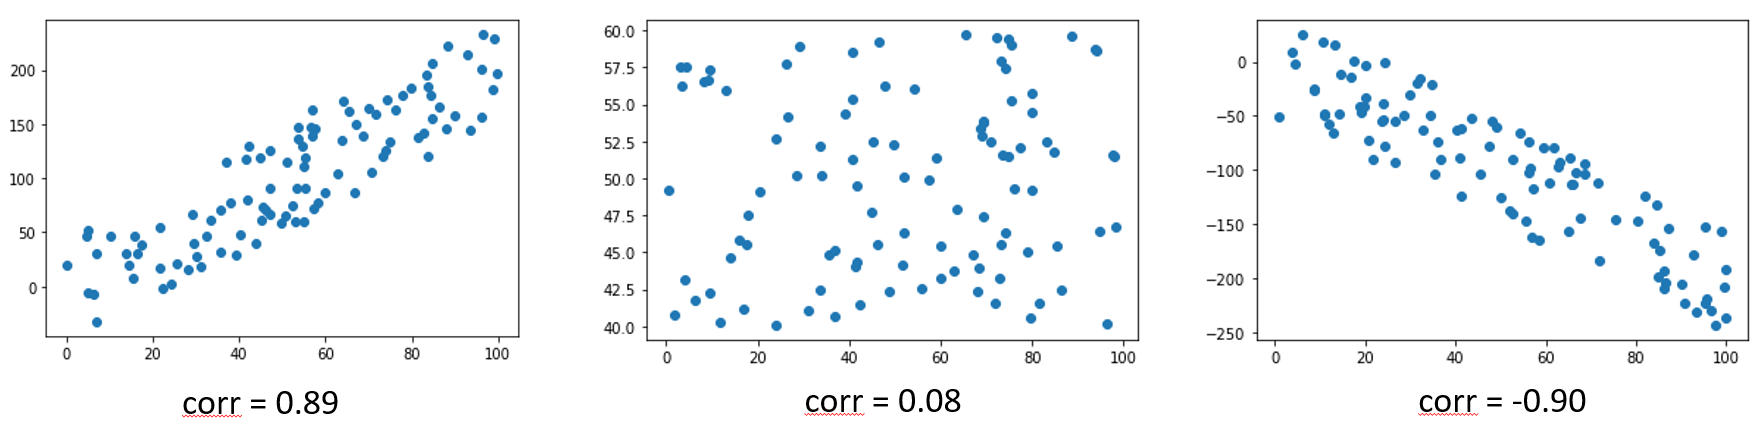
\includegraphics[keepaspectratio]{images/image10.png}}}

\subsubsection{\texorpdfstring{{Distribuzioni discrete e
continue}}{Distribuzioni discrete e continue}}\label{h.qm5j0el6gd7o}

{Nelle discrete ogni risultato univoco è assegnata una probabilità,
nelle continue ogni valore può assumere tutti i valori in un certo
intervallo, quindi non possiamo associare ad ogni valore preciso una
percentuale ma la assoceremo ad un range di valori.}

{}

{Alcuni esempi di discreta sono:}

\begin{itemize}
\tightlist
\item
  {Distribuzione uniforme}{: ogni variabile ha la stessa probabilità di
  assumere qualsiasi valore all\textquotesingle interno di un intervallo
  specificato, es: lancio di un dado, ogni faccia ha la stessa \% di
  uscita.}
\item
  {Distribuzione binomiale:}{~distribuzione del possibile numero di
  esiti positivi in un dato numero di prove in ciascuna delle quali
  esiste la stessa probabilità di successo.}
\end{itemize}

{}

{Alcuni esempi di continue:}

\begin{itemize}
\tightlist
\item
  {Normal }{distribution}{:}{~o gaussiana, è simmetrico rispetto alla
  media, mostrando che i dati vicini alla media sono più frequenti
  rispetto ai dati lontani dalla media. Sostanzialmente ha la seguente
  proprietà: se partendo dalla media tolgo o aumento una deviazione
  standard avrò un intervallo dove si avrà il 68,3 \% della popolazione,
  se mi sposto di due deviazioni avrò il 95.4\% della popolazione.}
\end{itemize}

{\pandocbounded{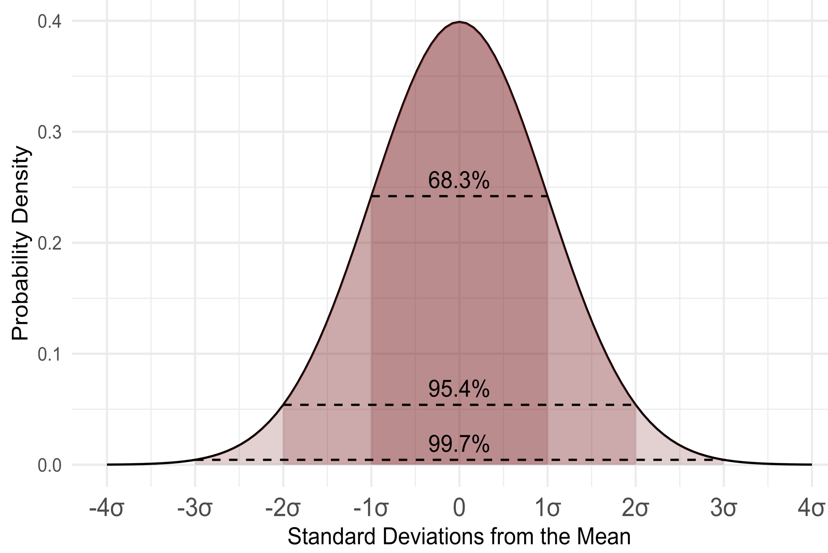
\includegraphics[keepaspectratio]{images/image7.png}}}

{Di sotto c'è la tabella che rappresenta di quanto dobbiamo aggiungere o
togliere per avere la percentuale di popolazione:}

{\pandocbounded{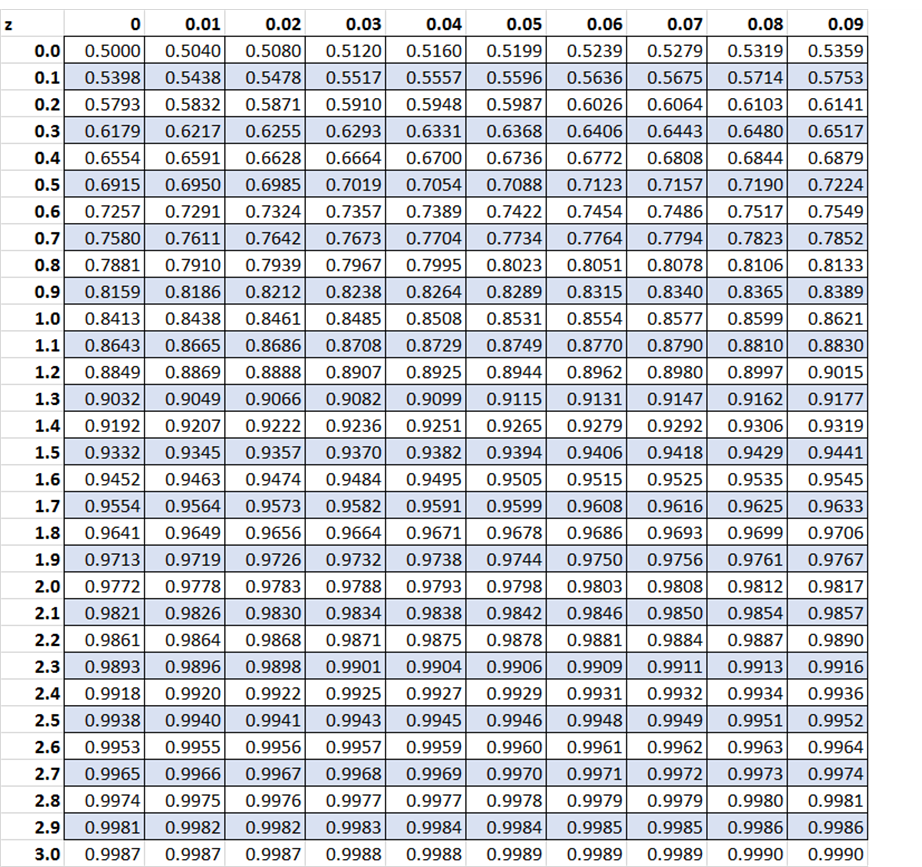
\includegraphics[keepaspectratio]{images/image9.png}}}

\section{\texorpdfstring{{Popolazione e
campione}}{Popolazione e campione}}\label{h.x17k06gzwyli}

{\pandocbounded{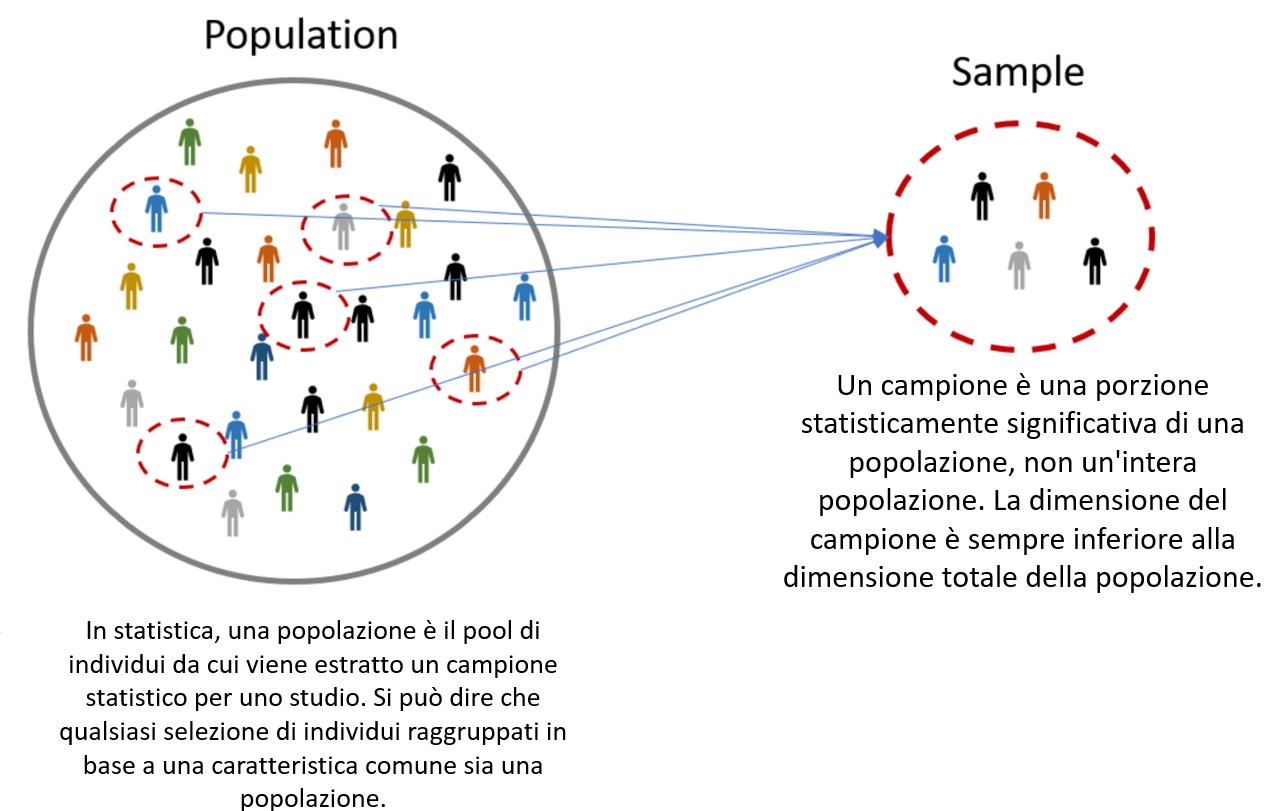
\includegraphics[keepaspectratio]{images/image8.png}}}

{}

\section{\texorpdfstring{{Teorema del limite
centrale}}{Teorema del limite centrale}}\label{h.hisdhmbnkc1m}

{Prendendo un insieme di campioni random da una popolazione più grande e
facendo la media otterremo un valore che va bene anche per l'intera
popolazione, questo è vero grazie a questo teorema.}

{}

{Prendendo più campioni e facendo sempre le medie e mettendole tutte in
un grafico queste si distribuiranno tramite una gaussiana/distribuzione
normale e non importa com'era la distribuzione di partenza.}

{}

\section{\texorpdfstring{{Errore
standard}}{Errore standard}}\label{h.hygy2hbi8yih}

{Se nel teorema precedente prendiamo campioni sempre più piccoli la
media risultante sarà affetta da un errore sempre più grande, al
contrario più il campione è grande più l'errore diminuisce.}

{}

{L'errore standard segue la formula: }

{deviazione standard / radice del numero di campioni}

{}

\section{\texorpdfstring{{Intervalli e livelli di
confidenza}}{Intervalli e livelli di confidenza}}\label{h.dur3152linaf}

{Come detto prima se dalla media ci spostiamo di + o - due (1.960 per
l\textquotesingle esattezza) valori dalla deviazione standard avremo il
95\% circa della popolazione, quindi abbiamo la sicurezza che ad ogni
calcolo al 95\% la media cada la dentro, ma è possibile che un campione
cadi fuori con una percentuale del 5\%}

{}

{L'intervallo di confidenza è un range, che va dalla media - l'errore
alla media + l'errore, con la media nel mezzo,
all\textquotesingle interno del quale si stima che possa trovarsi il
vero valore di un parametro di interesse. Il livello invece è la
probabilità, che la media calcolata tramite campione ha, di cadere lì
dentro.}

{}

{Per trovare l'intervallo c'è la formula:}

\pandocbounded{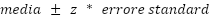
\includegraphics[keepaspectratio]{images/image1.png}}

{dove la z la prendiamo dalla tabella in modo da ottenere la percentuale
voluta che il valore cada dentro l'intervallo. }

{Quindi usando la formula otteniamo due valori (uno calcolando con il +
l'altro con il -) che sono gli estremi dell'intervallo che ha la
percentuale, data da z, di quanto un valore possa cadere lì dentro.}

{}

\section{\texorpdfstring{{Test di
ipotesi}}{Test di ipotesi}}\label{h.6dqzqwxadnhx}

{Serve per verificare che un dato ottenuto da una popolazione sia
effettivamente significativo.}

{I passaggi sono:}

\begin{itemize}
\tightlist
\item
  {imporre l'ipotesi nulla}{: il caso base, se per esempio vogliamo
  valutare se i tiri con i dadi che abbiamo fatto siano veri l'ipotesi
  nulla è dire che il dado sia regolare e che quindi tutte le facce
  escano con la stessa frequenza;}
\item
  {settare un livello di significabilità
  }\pandocbounded{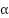
\includegraphics[keepaspectratio]{images/image2.png}}{:
  per esempio voglio essere sicuro al 95\% quindi alfa sarà 95:}
\item
  {calcolo la probabilità}{: il p-value, cioè quanto è raro che il
  risultato ottenuto possa avvenire.}
\end{itemize}

{}

{Per concludere se il p-value \textless{}
}\pandocbounded{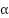
\includegraphics[keepaspectratio]{images/image2.png}}{~allora
posso rifiutare/rigettare l'ipotesi nulla.}

{\pandocbounded{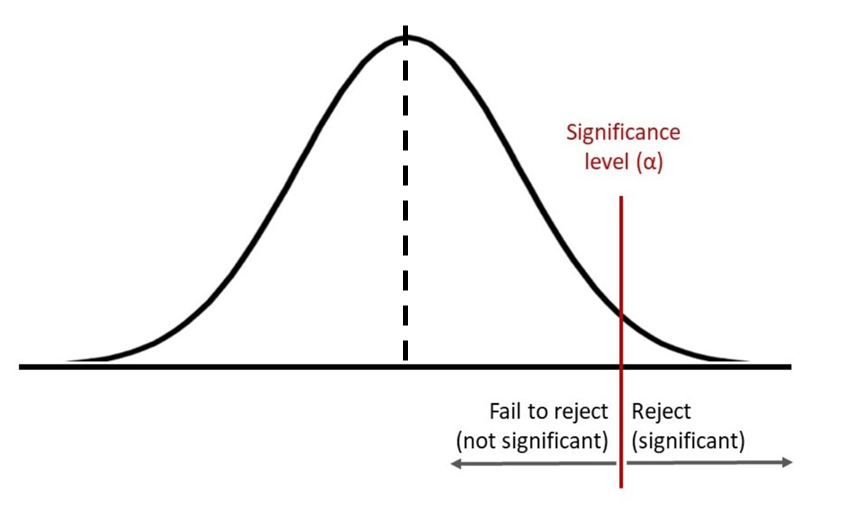
\includegraphics[keepaspectratio]{images/image11.png}}}

{I test sono diversi e si differenziano in aspetti come il numero di
campioni, e sono:}

\begin{itemize}
\tightlist
\item
  {T-test:}{~confrontare due gruppi/categorie di variabili numeriche con
  un campione di piccole dimensioni}
\item
  {Z-test: }{confrontare due gruppi/categorie di variabili numeriche con
  un campione di grandi dimensioni}
\item
  {ANOVA test}{: confrontare la differenza tra due o più
  gruppi/categorie di variabili numeriche}
\item
  {Chi-Squared test}{: esaminare la relazione tra due variabili
  categoriche}
\item
  {Correlation test}{: esaminare la relazione tra due variabili
  numeriche}
\end{itemize}

{}

{}

{Regressione lineare}

{Fa parte del machine learning supervisionato, quindi forniamo l'input e
label cioè la descrizione dell'input.}

{In questo caso abbiamo variabili indipendenti e fornisco l'output
atteso in modo da allenare il modello.}

{}

{La regressione lineare è un modello che cerca di trovare la relazione
fra più variabili indipendenti e una variabile dipendente. Nel dettaglio
il modello va a trovare la retta che descrive meglio la relazione fra i
valori, quindi il coefficiente della retta che si avvicina di più ai
valori sullo scatter plot.}

{}

{Quindi avremo una funzione:}

\pandocbounded{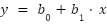
\includegraphics[keepaspectratio]{images/image3.png}}

{Dove:}

\begin{itemize}
\tightlist
\item
  {y}{: variabile dipendente}
\item
  {x}{: variabili indipendente}
\item
  \pandocbounded{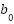
\includegraphics[keepaspectratio]{images/image4.png}}{:
  intercetta, l'alzata all'origine cioè dove l'x è 0 }{l'y}{~assume il
  valore di 0}
\item
  \pandocbounded{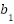
\includegraphics[keepaspectratio]{images/image5.png}}{:
  coefficiente angolare, la pendenza della retta e dice la variazione
  delle x al variare delle y.}
\end{itemize}

{}

{Per individuare questa retta è definita una }{Cost function}{, che dà
la somma delle misure fra la distanza dei punti e la retta (fra y e y)
al quadrato diviso poi il numero di punti.}

{L'obiettivo del modello sarà poi quello di trovare i coefficienti in
modo che la cost function sia la più piccola possibile.}

{}

{Esiste l'}{R quadro }{che serve per capire la bontà del modello, per
farlo calcoliamo la distanza fra i punti e la retta tracciata nel punto
medio di y, perché se i punti sono distanti tra loro senza correlazione
la retta creata dal modello non sarà mai buona come quella della media;
in sostanza:}

{Se la retta è buona
}\pandocbounded{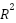
\includegraphics[keepaspectratio]{images/image6.png}}{~è
uguale a 1 }

{}

{}

{Time series}

{Nell\textquotesingle analizzare le serie storiche possiamo farlo in due
modi: con scomposizione o modellistica (usato da noi).}

{}

{Una serie storica è stazionaria se non c'è correlazione con il tempo e
se oscilla tra un medesimo valore, inoltre non ci devono essere trend e
stagionalità.}

{}

{Nella funzione di autocorrelazione globale, detta anche ACF, i picchi
determinano una correlazione fra ogni variabile della serie e k valori
indietro. }

{Per esempio un }{picco}{~su 1 indica che c'è correlazione tra ogni
valore della serie e il valore precedente, se c'è sul 2 indica che c'è
correlazione tra ogni valore della serie e il valore che }{ricorre
due}{~valori precedenti.}

{}

{}

\end{document}
